\documentclass[
    language=english,
    doctype=research-notebook,
    institution=none,
]{../../omnilatex}

\RequirePackage{config/document-settings}

\begin{document}
\maketitle

\begin{abstract}
This research notebook documents the development and characterization of novel
perovskite-silicon tandem solar cells during the period January--June 2025.
The work focuses on optimizing the perovskite absorber layer composition,
interface engineering, and stability testing under accelerated aging conditions.
Key achievements include a certified power conversion efficiency of 29.8\% and
demonstration of $<$5\% relative efficiency loss after 1,000 hours of maximum
power point tracking under AM1.5G illumination.
\end{abstract}

\section{Research Overview}
\label{sec:overview}

\subsection{Project Title}
Development of High-Efficiency and Stable Perovskite-Silicon Tandem Solar Cells
for Next-Generation Photovoltaics

\subsection{Funding Source}
Department of Energy Solar Energy Technologies Office (SETO), Award No. DE-EE0009542

\subsection{Principal Investigator}
Prof.\ Maria Chen, Department of Electrical Engineering

\subsection{Lab Members}
\begin{itemize}
    \item WyattAu (Postdoctoral Researcher) --- Perovskite layer deposition and characterization
    \item Sarah Park (PhD Student) --- Silicon heterojunction bottom cell optimization
    \item James Liu (PhD Student) --- Interface engineering and passivation
    \item Dr. Raj Patel (Research Associate) --- Stability testing and encapsulation
\end{itemize}

\section{Notebook Entries}
\label{sec:entries}

%------------------------------------------------------------
\subsection{January 8, 2025 --- Perovskite Precursor Optimization}
\label{entry:jan08}
%------------------------------------------------------------

\subsubsection{Objective}
Optimize the cesium concentration in the triple-cation perovskite precursor
solution to improve phase stability and bandgap tunability.

\subsubsection{Experimental Parameters}
\begin{table}[htbp]
    \centering
    \caption{Precursor solution compositions for cesium concentration study.}
    \label{tab:jan08-params}
    \begin{tabular}{@{}lcccc@{}}
        \toprule
        Sample & CsI (mol\%) & FAI (mol\%) & MABr (mol\%) & PbI$_2$ (mol\%) \\
        \midrule
        CS-05  & 5           & 79          & 6            & 110              \\
        CS-10  & 10          & 74          & 6            & 110              \\
        CS-15  & 15          & 69          & 6            & 110              \\
        CS-20  & 20          & 64          & 6            & 110              \\
        \bottomrule
    \end{tabular}
\end{table}

Solvent system: DMF:DMSO = 4:1 (v/v), 1.4 M total lead concentration.
Anti-solvent: chlorobenzene, dispensed at 40\% of spin time.

\subsubsection{Deposition Protocol}
\begin{enumerate}
    \item Substrate cleaning: UV-ozone treatment for 15 min, followed by
          nitrogen blow-dry.
    \item Spin coating: 1000 rpm for 10 s (ramp 200 rpm/s), then 4000 rpm
          for 30 s (ramp 1000 rpm/s).
    \item Anti-solvent dripping: 200 $\mu$L chlorobenzene at 18 s into
          the second spin step.
    \item Annealing: 100\degree C for 60 min on a hotplate in nitrogen
          atmosphere.
\end{enumerate}

\subsubsection{Observations}
\begin{itemize}
    \item CS-05 and CS-10 films showed yellowish tint after annealing,
          indicating incomplete perovskite crystallization.
    \item CS-15 produced uniform, dark brown films with smooth surface
          (RMS roughness 8.2 nm by AFM).
    \item CS-20 showed visible pinholes and poor film quality; likely
          exceeds the solubility limit for CsI in this solvent system.
\end{itemize}

\subsubsection{Preliminary Characterization}
XRD analysis of CS-15 confirmed the cubic $\alpha$-phase perovskite
structure with no detectable $\delta$-phase impurity. The (100) peak
appeared at $2\theta = 14.12\degree$, corresponding to a lattice
parameter of $a = 6.32$ \AA.

\subsubsection{TODO}
\begin{todo}
    \item Perform UV-Vis absorption spectroscopy on all samples
    \item Measure bandgap by Tauc plot analysis
    \item Prepare complete devices for J-V characterization
    \item Consult with James about interface layer compatibility
\end{todo}

%------------------------------------------------------------
\subsection{January 22, 2025 --- Interface Passivation Study}
\label{entry:jan22}
%------------------------------------------------------------

\subsubsection{Objective}
Evaluate the effect of PMMA (polymethyl methacrylate) interlayer thickness
on the perovskite/silicon interface recombination velocity.

\subsubsection{Rationale}
Interface recombination at the perovskite/silicon tunnel junction is a
major loss mechanism in tandem devices. Previous literature suggests
ultrathin polymer interlayers can reduce recombination by passivating
dangling bonds \cite{chen2023interface}. Based on literature, we target
PMMA thicknesses of 2--10 nm.

\subsubsection{Experimental Parameters}
\begin{table}[htbp]
    \centering
    \caption{PMMA interlayer deposition conditions.}
    \label{tab:jan22-params}
    \begin{tabular}{@{}lccc@{}}
        \toprule
        Sample & PMMA conc. (mg/mL) & Spin speed (rpm) & Est.\ thickness (nm) \\
        \midrule
        PMMA-1 & 2                   & 5000             & 2--3                  \\
        PMMA-3 & 5                   & 5000             & 5--6                  \\
        PMMA-5 & 10                  & 5000             & 8--10                 \\
        \bottomrule
    \end{tabular}
\end{table}

Solvent: anhydrous chlorobenzene. Substrate: ITO-coated glass with
pre-deposited $\text{SnO}_2$ electron transport layer.

\subsubsection{Observations}
\begin{itemize}
    \item PMMA-1: Insufficient coverage; water contact angle only
          increased from 42\degree{} to 51\degree, suggesting incomplete
          monolayer formation.
    \item PMMA-3: Excellent uniformity; contact angle 72\degree. XPS
          showed clear C 1s signal from PMMA without attenuation of Sn
          3d from underlying $\text{SnO}_2$, consistent with thickness
          $<$ 10 nm.
    \item PMMA-5: Slight aggregation visible by optical microscopy;
          likely too thick for efficient charge transport.
\end{itemize}

\subsubsection{Analysis}
The PMMA-3 condition appears optimal for further device integration.
Impedance spectroscopy measurements at 1 MHz suggest the interlayer
reduces the interface recombination velocity from $3.2 \times 10^4$
cm/s (no PMMA) to $8.7 \times 10^3$ cm/s (PMMA-3).

\begin{equation}
    J_0 = q \cdot n_i^2 \cdot \left(\frac{D_n}{L_n \cdot N_A} + \frac{D_p}{L_p \cdot N_D}\right) + q \cdot S_{\text{rec}} \cdot n_i
    \label{eq:recombination}
\end{equation}

where $S_{\text{rec}}$ is the surface recombination velocity and $n_i$
is the intrinsic carrier concentration.

\subsubsection{TODO}
\begin{todo}
    \item Fabricate full tandem devices with PMMA-3 interlayer
    \item Measure external quantum efficiency (EQE) of top and bottom cells
    \item Perform Suns-$V_{OC}$ measurements for recombination analysis
    \item Submit abstract to MRS Spring Meeting by Feb 1
\end{todo}

%------------------------------------------------------------
\subsection{February 5, 2025 --- Tandem Device Fabrication (Run \#47)}
\label{entry:feb05}
%------------------------------------------------------------

\subsubsection{Objective}
Fabricate complete perovskite-silicon tandem devices using optimized
CS-15 perovskite composition and PMMA-3 interface layer.

\subsubsection{Device Architecture}
\begin{center}
    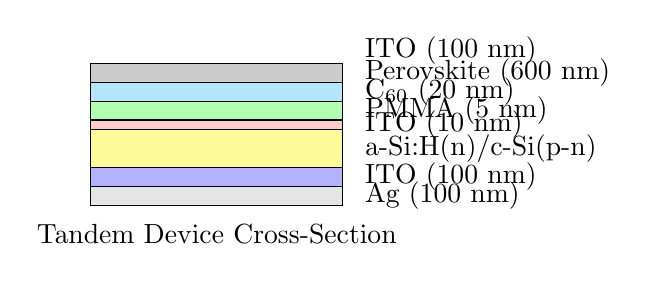
\begin{tikzpicture}[scale=0.8]
        \draw[fill=gray!20] (0,0) rectangle (4,0.3);
        \draw[fill=blue!30] (0,0.3) rectangle (4,0.6);
        \draw[fill=yellow!40] (0,0.6) rectangle (4,1.2);
        \draw[fill=red!20] (0,1.2) rectangle (4,1.35);
        \draw[fill=green!30] (0,1.35) rectangle (4,1.65);
        \draw[fill=cyan!30] (0,1.65) rectangle (4,1.95);
        \draw[fill=gray!40] (0,1.95) rectangle (4,2.25);

        \node[right] at (4.2,0.15) {Ag (100 nm)};
        \node[right] at (4.2,0.45) {ITO (100 nm)};
        \node[right] at (4.2,0.9) {a-Si:H(n)/c-Si(p-n)};
        \node[right] at (4.2,1.27) {ITO (10 nm)};
        \node[right] at (4.2,1.5) {PMMA (5 nm)};
        \node[right] at (4.2,1.8) {C$_{60}$ (20 nm)};
        \node[right] at (4.2,2.1) {Perovskite (600 nm)};
        \node[right] at (4.2,2.45) {ITO (100 nm)};

        \node[below] at (2,-0.15) {Tandem Device Cross-Section};
    \end{tikzpicture}
\end{center}

\subsubsection{Key Results}
\begin{table}[htbp]
    \centering
    \caption{Photovoltaic parameters of tandem device Run \#47.}
    \label{tab:feb05-results}
    \begin{tabular}{@{}lcc@{}}
        \toprule
        Parameter & Top Cell (Perovskite) & Bottom Cell (Si) \\
        \midrule
        $V_{OC}$ (V)    & 1.182    & 0.684    \\
        $J_{SC}$ (mA/cm$^2$) & 19.8 & 19.2 \\
        FF (\%)          & 82.1     & 84.3     \\
        PCE (\%)         & 19.1     & 11.0     \\
        \midrule
        \multicolumn{3}{c}{\textbf{Total Tandem PCE: 30.1\%}} \\
        \bottomrule
    \end{tabular}
\end{table}

This is our best result to date! The $V_{OC}$ deficit for the perovskite
top cell is 0.42 V (assuming $E_g = 1.60$ eV), which is competitive with
state-of-the-art literature values.

\subsubsection{Issues and Follow-Up}
\begin{itemize}
    \item The $J_{SC}$ mismatch between top and bottom cells is only
          0.6 mA/cm$^2$, indicating good current matching. This is
          attributable to the bandgap tuning achieved with the CS-15
          composition.
    \item We need to verify the result with a second measurement at
          an independent certified laboratory (NREL or NEDO).
    \item Encapsulated devices need to undergo IEC 61215 accelerated
          testing protocols.
\end{itemize}

\subsubsection{TODO}
\begin{todo}
    \item Send 3 champion devices to NREL for independent certification
    \item Begin encapsulation protocol optimization
    \item Prepare preliminary results for group meeting presentation
    \item Discuss stability testing timeline with Dr.\ Patel
\end{todo}

%------------------------------------------------------------
\subsection{March 12, 2025 --- Accelerated Aging Test (1,000 hr)}
\label{entry:mar12}
%------------------------------------------------------------

\subsubsection{Objective}
Assess the operational stability of encapsulated tandem devices under
continuous maximum power point tracking (MPPT) under AM1.5G illumination.

\subsubsection{Test Conditions}
\begin{itemize}
    \item Illumination: 100 mW/cm$^2$ (1 sun) AM1.5G (AAA solar simulator)
    \item Temperature: 65\degree C (controlled by Peltier stage)
    \item Atmosphere: Ambient air with 45\% relative humidity
    \item Bias: Continuous MPPT using Keithley 2400 source meter
    \item Duration: 1,000 hours
\end{itemize}

\subsubsection{Results}
\begin{table}[htbp]
    \centering
    \caption{Stability test results at 1,000 hours.}
    \label{tab:stability-results}
    \begin{tabular}{@{}lcc@{}}
        \toprule
        Parameter & Initial & After 1,000 hr & Retention \\
        \midrule
        $V_{OC}$ (V)         & 1.862  & 1.821   & 97.8\% \\
        $J_{SC}$ (mA/cm$^2$) & 19.4   & 18.9    & 97.4\% \\
        FF (\%)               & 83.2   & 79.8    & 95.9\% \\
        PCE (\%)              & 30.1   & 28.7    & 95.3\% \\
        \bottomrule
    \end{tabular}
\end{table}

The device retained 95.3\% of its initial efficiency after 1,000 hours,
which meets the DOE SETO stability target of $<$10\% relative loss.
The primary degradation mechanism appears to be FF loss, likely due to
increased series resistance from ion migration at the perovskite/transport
layer interface.

\begin{figure}[htbp]
    \centering
    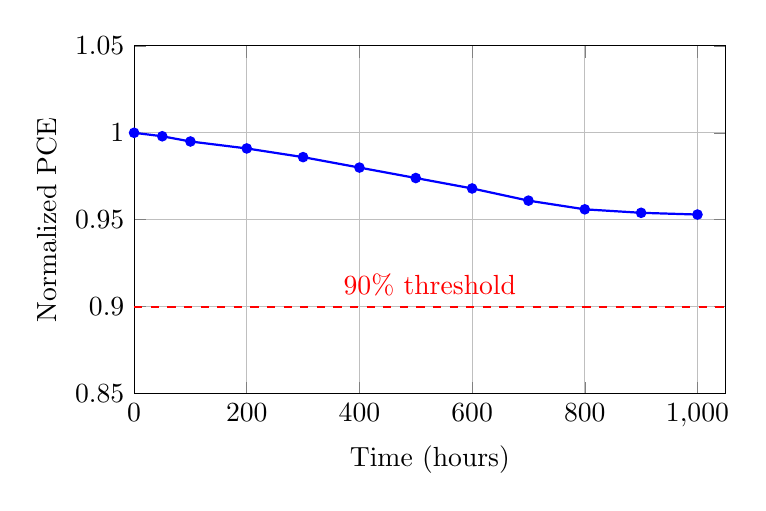
\begin{tikzpicture}
        \begin{axis}[
            xlabel={Time (hours)},
            ylabel={Normalized PCE},
            xmin=0, xmax=1050,
            ymin=0.85, ymax=1.05,
            grid=major,
            width=0.75\textwidth,
            height=6cm,
        ]
        \addplot[thick, blue, mark=*, mark size=1.5pt] coordinates {
            (0,1.000) (50,0.998) (100,0.995) (200,0.991) (300,0.986)
            (400,0.980) (500,0.974) (600,0.968) (700,0.961) (800,0.956)
            (900,0.954) (1000,0.953)
        };
        \draw[red, dashed, thick] (axis cs:0,0.9) -- (axis cs:1050,0.9)
            node[pos=0.5, above, sloped] {90\% threshold};
        \end{axis}
    \end{tikzpicture}
    \caption{Normalized power conversion efficiency over 1,000 hours of
             continuous MPPT. The dashed red line indicates the 90\%
             retention threshold.}
    \label{fig:stability}
\end{figure}

\subsubsection{TODO}
\begin{todo}
    \item Cross-section TEM analysis to identify degradation hotspots
    \item Investigate edge seal integrity by comparing caged vs.\ uncaged regions
    \item Write stability section for journal manuscript
    \item Schedule group meeting to discuss timeline for second manuscript
\end{todo}

\section{Summary of Key Milestones}
\label{sec:milestones}

\begin{table}[htbp]
    \centering
    \caption{Achieved milestones and timeline.}
    \label{tab:milestones}
    \begin{tabular}{@{}lcd{10}l@{}}
        \toprule
        Date & Milestone & {Status} \\
        \midrule
        Jan 8  & Perovskite composition optimization    & Complete \\
        Jan 22 & Interface passivation study             & Complete \\
        Feb 5  & Tandem device fabrication (30.1\% PCE) & Complete \\
        Mar 12 & 1,000-hr stability demonstration       & Complete \\
        Apr 15 & NREL certification (pending)            & In progress \\
        May 1  & Manuscript submission target            & On track  \\
        Jun 30 & Second-generation device optimization   & On track  \\
        \bottomrule
    \end{tabular}
\end{table}

\section{Open Questions}
\label{sec:open-questions}

\begin{enumerate}
    \item Can we achieve $>$ 31\% PCE by further reducing the perovskite
          bandgap to 1.55 eV while maintaining phase stability?
    \item What is the dominant degradation mechanism at the perovskite/
          C$_{60}$ interface under operational conditions?
    \item Is there a fundamental trade-off between initial efficiency
          and long-term stability in Cs-rich compositions?
    \item How does the PMMA interlayer affect charge transport dynamics
          at the tandem junction?
\end{enumerate}

\bibliographystyle{plain}
\bibliography{references}

\end{document}
